\documentclass{article}
\usepackage{../../std_header}

\begin{document}
	\title{Games in Extensive Form and Congestion Games}
	\author{Haoran Peng}
	\maketitle
In a strategic game, players make their moves simultaneously. In an extensive form game, players make moves in sequence. An example game tree is shown below (taken from Kousha's slides):
\begin{figure}[hbt!]
\centering
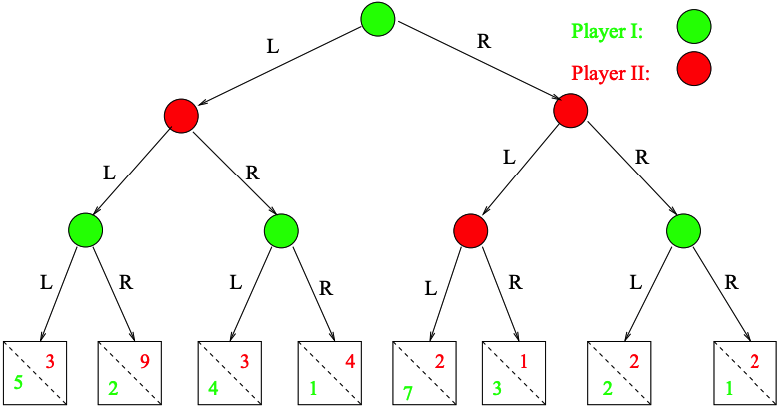
\includegraphics[width=.7\textwidth]{figs/tree1}
\end{figure}
A game tree can also include chance nodes (where the nature rolls a dice) and information sets. Nodes in the same information set is indistinguishable, and thus all those nodes need to make the same move in a strategy.
\begin{figure}[hbt!]
	\centering
	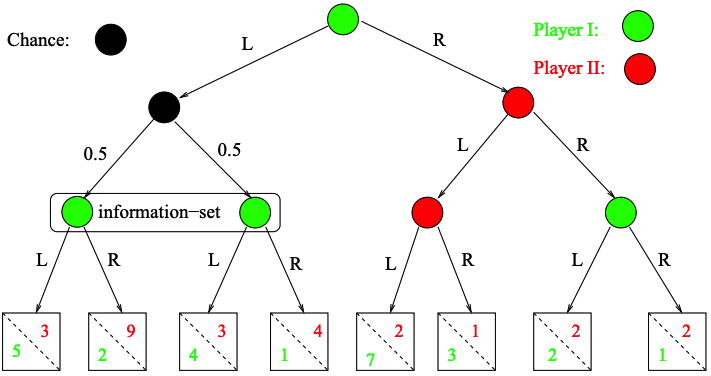
\includegraphics[width=.7\textwidth]{figs/tree2}
\end{figure}

The formal definition of an extensive game is omitted, not very useful in understanding the concept.

An extensive form game is a game of \textbf{imperfect} (but complete information, we will talk about incomplete information games later) if it has information sets with size > 1. The first game tree is a game of perfect information while the second is a game of imperfect information.

A game has \textbf{perfect recall} if whenever two nodes $w, w'$ are in the same information set for player $i$, the prior sequence of informations sets and actions taken prior to hitting node $w$ or node $w'$ must be the same. 

With perfect recall, it suffices to restrict player's strategies to \textbf{behaviour strategies}. Where randomization only happens at each information set (and no randomization of the whole strategy).
\\~\\
\textbf{Subgame and subgame perfection}

A subgame is any subtree of a game with self-contained information sets.

A strategy profile is a \textbf{subgame perfect Nash equilibrium (SPNE)} of game $\mathcal{G}$ if it defines an NE in every subgame of $\mathcal{G}$.

\textbf{Kuhn's Theorem: } Every finite $n$-person perfect information game $\mathcal{G}$ has a subgame perfect Nash equilibrium in \textbf{pure} strategies. This can be proved using induction (backward induction).

\newpage
\textbf{Congestion game}

A congestion game has:
\begin{itemize}
\item A finite set $N = \{1,\ldots,n\}$ of players
\item A finite set $R = \{1, \ldots,m\}$ of resources
\item For each player, $i$, a set $Z_i \subseteq 2^R$ of admissible strategies. So a pure strategy of $s_i\in Z_i$ is a set of resources.
\item Each resource $r\in R$ has a cost function $d_r:\mathbb{N}\mapsto \mathbb{Z}$. If there are $j$ agents using resource $r$, the cost is $d_r(j)$.
\item For a pure strategy profile $s = (s_1, \ldots, s_n)$, the congestion on resource $r$ is $n_r(s) = |\{i\mid r \in s_i\}|$
\item Under profile $s$, the total cost to player $i$ is:
\begin{align*}
	C_i(s) = \sum_{r\in s_i} d_r(n_r(s))
\end{align*} 
\item Every player wants to minimize its own expected cost.
\end{itemize}


\textbf{Rosenthal's Theorem: } In any congestion game, every sequence of strict improvement steps is necessarily finite, and terminates in a \textbf{pure} Nash Equilibrium. Thus, in particular, every congestion game has a pure strategy Nash Equilibrium.

This means if we start with any pure strategy profile, and each player $i$ iteratively switch to a \textbf{strictly} better strategy (with lower cost) until no player can lower their cost, the final profile is a pure NE.
\\~\\
For the following networks, $x$ is the proportion of agents that use that edge (e.g. if there are $n$ agents and 5 use that edge $x=5/n$).

The NE for the network below is when all agents use the bottom edge. Because if some agents are using the top edge, they would switch to the bottom for a lower cost. Average cost in NE = 1. The global best is for half to use the top edge and another half to use the bottom edge, $1/2 + 1/2 \times 1/2 = 3/4$. The ratio between the NE cost and the global best is $1/(3/4) = 4/3$
\begin{figure}[hbt!]
	\centering
	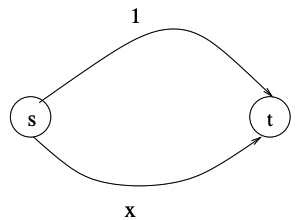
\includegraphics[width=.35\textwidth]{figs/flow1}
\end{figure}
\newpage
$d$ is some number > 1. The NE is still for all agents to go the bottom edge, for the same reason. If $d$ is large enough, the global best average cost can be less than any $\epsilon$ if we send all but one agents through the bottom and one through the top edge.
\begin{figure}[hbt!]
	\centering
	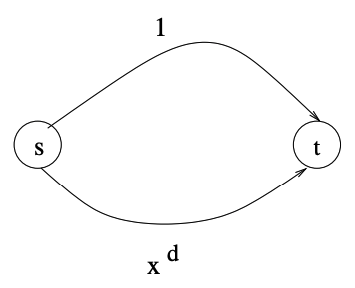
\includegraphics[width=.35\textwidth]{figs/flow2}
\end{figure}

Clearly, the NE and the global best is for half the agents to go the top route and half to go the bottom route. Average cost = $1/2 + 1 = 3/ 2$.
\begin{figure}[hbt!]
	\centering
	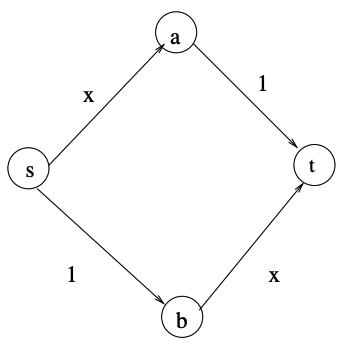
\includegraphics[width=.35\textwidth]{figs/flow3}
\end{figure}

Braess’s paradox: we add a superhighway link in the middle. The NE average cost is now 2, all of the agents will choose the x-0-x route, which is higher than without the highway.  The global best average cost is still $3/2$. The ratio between the NE cost and the global best is $2/(3/2) = 4/3$.
\begin{figure}[hbt!]
	\centering
	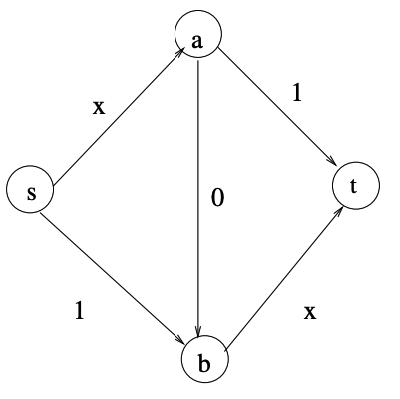
\includegraphics[width=.35\textwidth]{figs/flow4}
\end{figure}
\newpage
\textbf{Price of Anarchy}

We noticed that in congestion games, if we allow agents to choose their strategy selfishly (i.e. anarchy), the average cost is higher than we stipulate some best strategy profiles. And interestingly, the ratio between the NE cost and the global best average cost in  two of the examples are both $4/3$, and in one example this ratio can tend towards infinity.

It is shown that in a congestion game $\Gamma$ where \textbf{every edge's cost is a linear function of $x$} the worst case price of anarchy:
\begin{align*}
	\text{price-of-anarchy} = \frac{\max_{s \in S} \text{welfare}(s)}{\min_{s \in \text{NE}(\Gamma) \text{welfare}(s)}}
\end{align*}
is $4/3$, where welfare$(s) = 1/$average cost.

The pure price of anarchy for a \textbf{pure} NE in atomic (finite number of players) network congestion games with linear utilities is $5/2$.
\end{document}














